\chapter{Design}
\label{sec:design}
In this chapter the design for the Camera Provisioning system will be laid out.
The goal of the system is to provide a solution which makes it possible to manage camera configurations.
The system allows the user to orchestrate parameters into different templates which can be assinged to a camera.
The design will contain both functional and technical specifications containing the descriptions of different components, requirements and supplemental diagrams and wireframes.
\section{Requirements}
In table \ref{tab:requirements} the requirements for the system have been defined. Requirements are tracked using an identifier starting with a letter followed by a
number and are listed in the ID column of table \ref{tab:requirements}. If the identifier starts with the letter 'B' or a 'U' they specify a business or user requirement respectively. If the identifier starts with a 'F' or 'NF' they specify a functional or non-functional system requirement respectively.
\begin{table*}[h]
    \centering
    \begin{tabulary}{\linewidth}{CLL}
        \textbf{ID} & \textbf{Requirement} & \textbf{MoSCoW}
    %%% Business requirements
        \\ \hline %% Check this with NF-7
        B1 & A camera can be configured by the user without detailed knowledge about the model being used & Must
        \\ \hline
        B2 & A camera can be rolled back to a previous configuration & Must
        \\ \hline
        B3 & It should be known who last changed a template and at what time & Must
        \\ \hline
        B4 & Translated parameters that are scaled to a particular value should be tuneable & Should
        \\ \hline
        B5 & A camera can be queried to verify if it still configured according to its template & ????
    %%% User requirements
        \\ \hline
        U1 & A user can login using a username \& password & Could
        \\ \hline
        U2 & A user can change his password through the web interface & Could
        \\ \hline
        U3 & A user can configure a NTP server in a template & Should
        \\ \hline
        U4 & A user can configure the motion detection sensitivity in a template & Must
        \\ \hline
        U5 & A user can configure video quality in a template & Should
        \\ \hline
        U6 & A template can contain a parameter that is not present in any of its parents & Should
        \\ \hline
        U7 & A user can interface with the system using a webbrowser & Should
        \\ \hline
        U8 & A user can create a new template with a specified parent template & Must
        \\ \hline
        U9 & A user shall be able to trigger the configuration on one or all cameras according to their template & Must
    %%% System requirements
        \\ \hline
        NF-1 & Communication with cameras are authenticated through HTTP Basic or Digest & Must
        \\ \hline
        NF-2 & The system shall be implemented in Go & Must
        \\ \hline
        NF-3 & All code shall be covered by unit tests & Must
        \\ \hline
        NF-4 & Templates and camera configuration can be stored on disk using YAML files & Must
        \\ \hline
        NF-5 & Templates and camera configuration can be loaded from YAML files & Must
        \\ \hline %% TODO check this with Wouter. Not SMART
        NF-6 & APIs will be documented/verified using OpenAPI when appropriate & Should
        \\ \hline
        NF-7 & Camera configurations shall be represented in a generic way so that they can be applied to different cameras. & Must
    \end{tabulary}
    \caption{Requirements}
    \label{tab:requirements}
\end{table*}

\section{General design}
At the conclusion of this project the prototype is handed over to the back-end team of BauWatch.
Since they will be further developing the prototype into a production ready system the choice was made to implement the system in Go as that programming language is their preferred language for new products.

\section{Templates}
The provisioning server will have a user interface through which a template can be configured.
A template in the context of this system is a collection of lists containing camera configuration options.
Templates can be built up from different layers where each layer can override parameters from the layer above.
This allows the user to define a template that is shared by a large amount of cameras but still provides more fine-tuned control for certain situations.
These cameras would still use all the settings from the parent template but would have a different setting for camera sensitivity.

\subsection{Parameters}
%TODO: How are the templates kept in memory. Describe the parameter interface
%TODO: How will stuff look in the main application
TBD Once I figure out how to properly abstract them in Go.
At the moment only integer parameters are supported.

\subsection{Storing to file}
Templates are stored on disk as YAML according to the following format.
\lstinputlisting[language=yaml]{format.yaml}

\subsection{Reading from file}
Templates are stored on disk with the name of the parent. When this file is reloaded to instantiate a template the system must be able to discover its
parent by its name. This can be achieved using a breadth-first search of the template tree.
The operation of loading a template and linking these to their parent is described in figure \ref{fig:inserttemplate}.

\begin{figure}[h!]
	\centering
	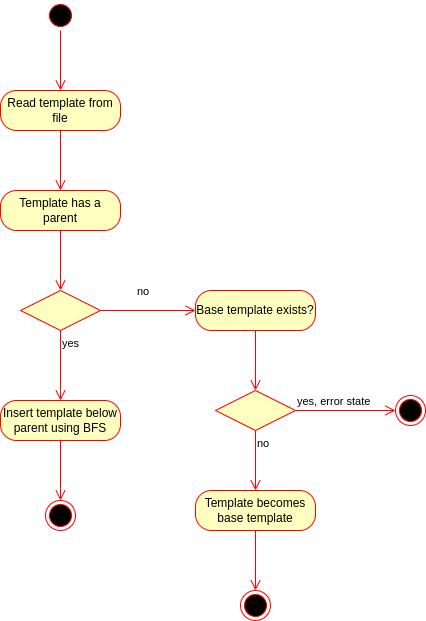
\includegraphics[scale=0.5]{insert_template_acty}
	\caption{Template insert operation}
	\label{fig:inserttemplate}
\end{figure}

\subsection{Keeping revision history}
In order to fullfill the ability to restore a template to a previous version a revision history is kept.
Templates are stored in a directory with the name of that template.
Inside that directory a template is stored as a file named with the revision number and the file extension (.yml).
This way the latest revision can be found by sorting the files by name in descending order.
When a template is reverted to a previous version the files will be sorted in the same manner and will be deleted until the revision to revert to is reached. An example of how this directory structure would be stored is seen in figure \ref{fig:diskstruct}

\begin{figure}[h!]
	\centering
	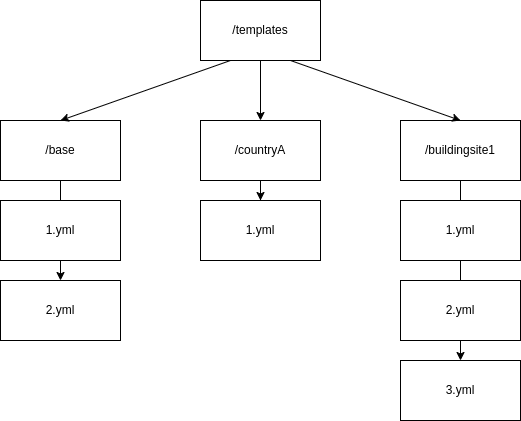
\includegraphics[scale=0.5]{yaml_dir_struct}
	\caption{Directory structure of templates and their revisions}
	\label{fig:diskstruct}
\end{figure}

\section{Camera interface}
The camera interface is a system component that sits between the template component and the cameras themselves. The purpose of this component
is to translate the settings from a template into an API call understood by the camera. Each camera can have a different API with potentially different interpretation of parameters. This component will map the parameter from the template to an appropriate value for that camera.
In order for a camera to accept new parameters they require a form of authentication. All cameras being used support both HTTP Basic and HTTP Digest authentication.
To successfully interface with the cameras one or both of these authentication methods must be supported by the camera interface component.

\section{Translating generic parameters to camera specific values}
Take sensitivity as an example. TBD

\section{User interface}
The components of the system can be managed through a web interface.
They will allow the user to create a new template and add parameters to it as seen in figure \ref{fig:templatewireframe}.
The user should also be able to manage the relations between templates as well as registering new cameras to be managed by the system (TBD still).
\begin{figure}[h!]
	\centering
	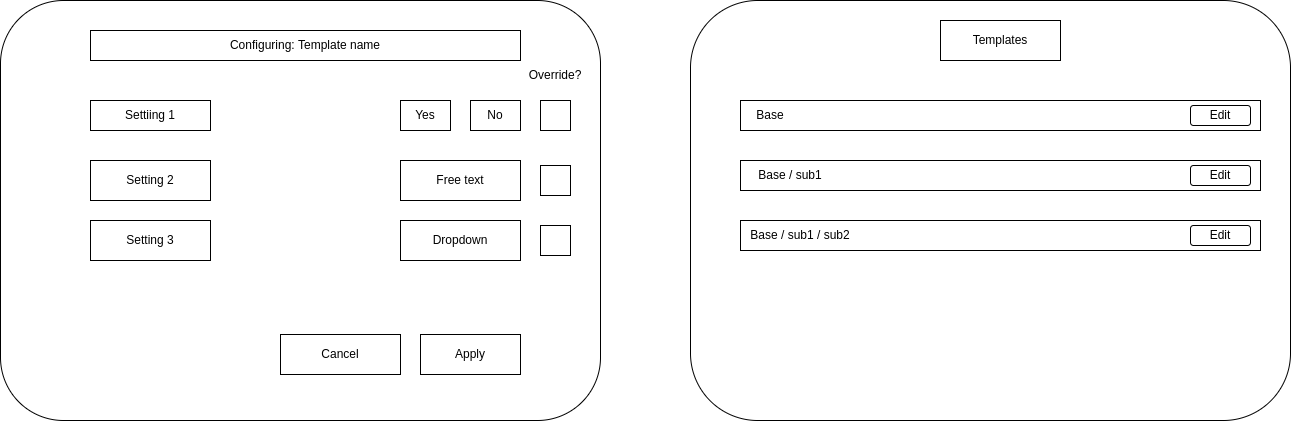
\includegraphics[scale=0.2]{wireframes}
	\caption{Template overview  wireframe}
	\label{fig:templatewireframe}
\end{figure}

\section{Design patterns}
TBD Integrate these where applicable instead of separately.

Design patterns are reusable solutions to commonly occurring software design problems. Design patterns are not ready made solutions that directly translate to machine readable code. Rather they are concepts that can be applied to solve a common problem in different situations. They may be seen as an intermediate between a programming paradigm (e.g. functional- or object-oriented programming) and
concrete algorithms. Design patterns can be divided in three categories, namely creational, behavioral and structural.

\subsection{Composite}
The composite pattern is a structural design pattern. With this design pattern objects can be grouped such that they are treated as a
single instance.

\subsection{Factory}
The factory method is a creational design pattern used for creating objects in a generic superclass that allows subclasses to change the
specific type of object that is created.
